% !TEX TS-program = xelatex
% !TEX encoding = UTF-8
%
%
\documentclass[a4paper,12pt]{article}
\usepackage{ctex}
\usepackage{geometry,anysize,changepage,calc,hyperref,cite,fancyhdr,setspace}
\usepackage{amsmath,amssymb,amsthm,listings,xcolor}
\usepackage{graphicx,wrapfig,multirow,diagbox,caption, subcaption,verbatim}
\usepackage{caption,algorithm,algpseudocode}
\usepackage{url,natbib}
\bibliographystyle{abbrvnat}
\setcitestyle{open={(},authoryear,close={)}}
\renewcommand{\algorithmicrequire}{\textbf{输入}}
\renewcommand{\algorithmicensure}{\textbf{输出}}
\floatname{algorithm}{子程序}
\listfiles
%initialset.tex
%
\hypersetup{bookmarksopen=true,colorlinks=true,linkcolor=red,anchorcolor=blue,citecolor=green,linktocpage=true}
\captionsetup{font=footnotesize}
\captionsetup[sub]{font+=footnotesize}
\linespread{1.5}
\marginsize{2.13cm}{2.14cm}{2.4cm}{2.4cm}
\pagestyle{fancy}
\lstset{xleftmargin=1.5em,xrightmargin=1.5em,frame=lines}%,numbers=left,numberstyle=\tiny}
\chead{}\rhead{\thepage}\lhead{\leftmark}\cfoot{}\rfoot{}\lfoot{}

\newcommand{\vp}{\varphi}
\newcommand{\al}{\alpha}
\newcommand{\be}{\beta}
\newcommand{\ti}{\tilde}
\newcommand{\ve}{\varepsilon}
\newcommand{\de}{\delta}
\newcommand{\na}{\nabla}
\newcommand{\pd}{\partial}
\newcommand{\ud}{\mathrm{d}}
\newcommand{\mr}{\mathrm{R}}
\newcommand{\ms}{\mathbb{S}}
\newcommand{\mz}{\mathbb{Z}}
\newcommand{\mn}{\mathbb{N}}
\newcommand{\mc}{\mathbb{C}}
\newcommand{\one}{\textbf{1}}
\newcommand{\prox}{\textbf{prox}}
\DeclareMathOperator*{\argmax}{argmax}
\DeclareMathOperator*{\argmin}{argmin}
%\DeclareMathOperator*{\logg}{log}
%\DeclareMathOperator*{\det}{det}
\DeclareMathOperator*{\tr}{tr}
\DeclareMathOperator*{\st}{s.t.}

\theoremstyle{nonumberplain}
%\theoremheaderfont{\itshape}
%\theorembodyfont{\upshape}
%\theoremseparator{.}
%\theoremsymbol{\ensuremath{\square}
\newtheorem{definition}{定义}
\newtheorem{theorem}{定理}
\newtheorem{lemma}{引理}
%\newtheorem{proof}{证明}

%\renewcommand{\figurename}{{\zihao{5}图}}
%\renewcommand{\tablename}{{\zihao{5}表}}
%\makeatletter %下面两个命令用于创建非浮动体图表的标题
%  \newcommand\figcaption{\def\@captype{figure}\caption} 
%  \newcommand\tabcaption{\def\@captype{table}\caption} 
%\makeatother
%%\renewcommand{\abstractname}{摘\ 要}
%\renewcommand{\contentsname}{目\ 录}
%\renewcommand{\refname}{参考文献}

%\renewcommand{\thetable}{\arabic{section}.\arabic{table}}
%\renewcommand{\thefigure}{\arabic{section}.\arabic{figure}}
%\renewcommand{\theequation}{\arabic{section}.\arabic{equation}}

\makeatletter\@addtoreset{table}{section}\@addtoreset{figure}{section}\@addtoreset{equation}{section}\makeatother




\linespread{1.5}
\author{龙子超}
\title{{\heiti {\zihao{3} 数学分析II-习题课}}}
\date{}
\begin{document}
\maketitle
%===================正文====================
%\begin{abstract}
%\begin{spacing}{1.0}
%
%\end{spacing}
%\end{abstract}

%\tableofcontents
%\newpage

\section*{2018-Feb-28}
\noindent 3. 设函数 $f(x)\in C([0,1])$ 且 $f(0)\neq f(1)$. 证明: 存在 $\xi\in(0,1)$ 不是 $f(x)$ 的极值点.

\noindent 证明(若在考试中下面的证明过程应该更规范): 不失一般性,我们考虑 $f(0)<f(1)$ 的情形, 记 $a_0=0,b_0=1$, 依题设有 $f(a_0)<f(b_0)$. 我们构造如下$\{a_n\},\{b_n\}$
\begin{algorithm}
  \begin{algorithmic}
    \State for $n=0,1,\cdots$
    \State \ \ \ \ find $x\in(a_n,b_n)$ s.t. $f(x)=\frac{f(a_n)+f(b_n)}{2}$
    \State \ \ \ \ if $x-a_n<b_n-x$
    \State \ \ \ \ \ \ \ \ find $y\in(a_n,x)$ s.t. $f(y)=\frac{f(a_n)+f(x)}{2}$
    \State \ \ \ \ else 
    \State \ \ \ \ \ \ \ \ find $y\in(x,b_n)$ s.t. $f(y)=\frac{f(x)+f(b_n)}{2}$
    \State \ \ \ \ set $a_{n+1}=\min(x,y),b_{n+1}=\max(x,y)$
  \end{algorithmic}
\end{algorithm}

容易证明
\begin{eqnarray*}
  &[1]&f(b_0)>f(b_1)>\cdots>f(b_n)>\cdots>\cdots>f(a_n)>\cdots>f(a_1)>f(a_0),\\
  &[2]&b_0>b_1>\cdots>b_n>\cdots>\cdots>a_n>\cdots>a_1>a_0,\\
  &[3]&|a_{n+1}-b_{n+1}|<\frac{|a_n-b_n|}{2}
\end{eqnarray*}
依据闭区间套定理, 存在$c$满足$a_n<c<b_n,\forall n\in \mn$, $\lim_n a_n=\lim_n b_n=c$, 这时根据$f$的连续性有$f(c)=\lim_n f(a_n)=\lim_nf(b_n)$, 从而进一步有
\[
  f(b_0)>f(b_1)>\cdots>f(b_n)>\cdots>f(c)>\cdots>f(a_n)>\cdots>f(a_1)>f(a_0),\\
\]

依据$c,f(c)$的上述性质可知$c$不是极值点.

\noindent 4. 设函数 $f(x)$ 在 $[a,b]$ 内任一点处的极限均为0. 问: $f(x)$ 在 $[a,b]$ 上可积吗?\\
提示: 先证明$\forall \varepsilon>0,$ 只存在有限个点 $x\in[a,b]$ 使得 $f(x)>\varepsilon$, 再依据积分的定义证明函数黎曼可积.

\noindent 5. 函数作图:
\[
x = \frac{t^3-t^2+2}{t}, 
y = \frac{t^3-1}{t+1}
\]
\begin{figure}[htbp]
  \centering
  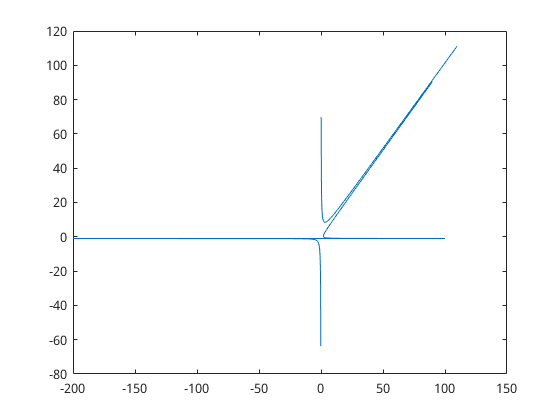
\includegraphics[width = 0.5\textwidth]{20180228_5.png}
  \caption{}
  \label{}
\end{figure}

\noindent 6. 设函数 $f(x):[0,1]\to [0,1]$ 连续, 函数 $g(x):[0,1]\to [0,1]$ 可积. 问: 复合函数 $f(g(x)),g(f(x))$ 在 $[0,1]$ 上是否可积?

\noindent 7. 设函数 $f(x)$ 在 $x=0$ 处满足 $f(x)=a_0+a_1x+\cdots+a_nx^n+o(x^n),x\to 0,n\geq1$. 问: $f(x)$ 在 $x=0$ 处是否存在直至 $n$ 阶导数? 若存在,请计算相应导数值.\\
提示: 取$f(x)=x^{n+1}\sin\frac{1}{x^{n+2}}$分$n=1$和$n>1$讨论.

\noindent 8. 设 $f(x)$ 是 $R$ 上的可微非常值函数且满足 $\forall x\in R, f(f(x))=f(x)$. 问: $f(x)\equiv x$ 是否成立?

\noindent 9. 设函数
\(
f(x)=\left\{\begin{array}{ll}
\frac{1}{x}-[\frac{1}{x}], & x\in(0,1],\\
1,                         & x=0,
\end{array}\right.
\)
其中 $[z]$ 表示不超过 $z$ 的最大整数. 计算 $\int_0^1f(x)\mathrm{d}x$\\
提示: $\int_0^1=\sum_{n=1}^{\infty}\int_{1/(n+1)}^{1/n}$

\noindent 10. 设 $f(x)\in C^1([0,\pi])$ 且满足 $\int_0^\pi f(x)sin(x)\mathrm{d}x=\int_0^\pi f(x)cos(x)\mathrm{d}x=0$. 证明: 
$\forall \alpha \in \mathrm{R}, \exists \xi \in (0,\pi), $ s.t. $ f'(\xi)-\alpha f(\xi)=0$.\\
证明:令$G(x)=f'(x)-\alpha f(x)$是连续函数, 依题设
\begin{eqnarray*}
  \int_0^\pi G(x)sin(x)\ud x&=&\int_0^\pi f'(x)\sin(x)\ud x-\alpha f(x)\sin(x)\ud x\\
  &=&\int_0^\pi f'(x)\sin(x)\ud x\\
  &=&f(x)\sin(x)\vert_0^\pi-\int_0^\pi f(x)\cos(x)\ud x\\
  &=&0
\end{eqnarray*}
因此$G$不可能在$(0,\pi)$上恒大于0或恒小于0, 依据零点存在定理可知$G$有0点.

%\begin{algorithm}
%  \caption*{ADMM求解$\min_{X\succeq0}|X|_1,\st |SX-I|\leq\sigma$}
%  %  \caption{ADMM求解$\min_{X\succeq0}|X|_1,\st |SX-I|\leq\sigma$}\label{alg:ADMM}
%  \begin{algorithmic}
%    \Require $S,\sigma,\rho$
%    \Ensure $X,|X|_1$
%    \State \textbf{Repeat while not convergence}
%    \begin{enumerate}
%      \item  根据式(\ref{eq:updateW3_2}
%      $\sim$\ref{eq:updateZ3_2}),依次求$W^+,X^+,Y^+,Z^+$;
%      \item  根据式(\ref{eq:updateU3_2}),依次求${U^1}^+,{U^2}^+,{U^3}^+$;
%    \end{enumerate}
%    \Return $X,|X|_1$
%  \end{algorithmic}
%\end{algorithm}

%\begin{lstlisting}[language=Matlab,keywordstyle=\color{blue},commentstyle=\color{red!80!green!80!blue!80}, rulesepcolor=\color{red!50!green!50!blue!50},tabsize=4]
%
%\end{lstlisting}

%\begin{figure}[htbp!]
%\centering
%\makebox[\textwidth][c] {
%\includegraphics[width=0.9\paperwidth]{}
%}
%\caption{}\label{}
%\end{figure}
%
%\begin{figure}[htbp!]
%   \centering
%   \begin{subfigure}{.48\textwidth}
%	\centering
%	\includegraphics[width = \textwidth]{}
%	\caption{} \label{}
%   \end{subfigure} 
%   \begin{subfigure}{.48\textwidth}
%	\centering
%	\includegraphics[width = \textwidth]{}
%	\caption{} \label{}
%   \end{subfigure}
%   \caption{} \label{}
%\end{figure}

%\begin{table}[htbp!]
%\centering
%\caption{} 
%\begin{subfigure}{0.49\textwidth}
%   \centering
%   \caption{}
%   \begin{tabular}{}
%
%   \end{tabular}
%\end{subfigure}
%\begin{subfigure}{.49\textwidth}
%   \centering
%   \caption{} 
%   \begin{tabular}{}
%
%   \end{tabular}    
%\end{subfigure}
%\end{table}

%\begin{centering}
%\section*{致谢}\addcontentsline{toc}{section}{致谢}
%\end{centering}

%\newpage
%\begin{thebibliography}{}
%\addcontentsline{toc}{section}{参考文献}
%\bibitem{cite_ADMM}Boyd S, Parikh N, Chu E, et al. Distributed Optimization and Statistical Learning via the Alternating Direction Method of Multipliers[J]. Foundations \& Trends® in Machine Learning, 2011, 3(1):1-122.
%\bibitem{cite_FISTA}Beck A, Teboulle M. A Fast Iterative Shrinkage-Thresholding Algorithm for Linear Inverse Problems[J]. Siam Journal on Imaging Sciences, 2009, 2(1):183-202.
%\bibitem{cite_convexoptimization}Boyd S, Vandenberghe L. Convex Optimization[M]. Cambridge University Press, 2004.
%%\bibitem{cite_quasicrystalsgreen}刘有延,傅秀军.\emph{准晶体}[M]. 上海科技教育出版社,1999.
%\end{thebibliography}

\bibliography{ref}
\end{document}



